\documentclass[12pt]{article}
\usepackage[letterpaper, margin=1in]{geometry}
% \usepackage[a4paper, margin=1in]{geometry}
\usepackage[T1]{fontenc}
\usepackage{lmodern}
\usepackage{graphicx}
\usepackage{amsmath}
\usepackage{indentfirst}
\usepackage[hidelinks, bookmarks=true]{hyperref}
\usepackage[section]{placeins}
\usepackage[
    natbib=true,
    style=phys,
    biblabel=brackets,
    giveninits=true,
    abbreviate=false,
    doi=true,
    url=true,
    isbn=false,
    block=space
]{biblatex}
\addbibresource{references.bib}
\DeclareFieldFormat{titlecase}{#1} % Keep title case formatting
\usepackage{lineno}

\title{
    Search for an exotic Higgs boson decay to two pseudoscalar bosons with a four photon final state\\[0.2cm]
    \Large Candidacy Proposal
}
\author{\\[0.25cm]Sergi Castells\\[0.25cm] Advisors: Colin Jessop and Nancy Marinelli\\[0.75cm]}
\date{December 13, 2023}

\begin{document}
\maketitle
\linenumbers

\section{Introduction}
The Standard Model (SM) is our most accurate and complete model of the universe, but there are yet many questions left unanswered. The SM does not account for dark matter, gravity, neutrino masses, and more. The search for Beyond the Standard Model (BSM) physics is an important facet of high energy physics that is motivated, in part, by these open questions. One set of interesting BSM phenomena to explore is exotic Higgs boson decays, which can be achieved in theories with extended Higgs sectors. It is important to first understand why the Higgs sector is so interesting, however.\par

The Higgs sector of the SM plays a crucial role in generating masses for all elementary particles except neutrinos. Masses for elementary particles are generated during electroweak symmetry breaking when the Higgs field gains a non-zero VEV (vacuum expectation values) and $\text{SU(2)}_\text{L} \times U(1)_\text{Y}$ break into U(1)\textsubscript{EM}. The W and Z bosons gain their mass from the Higgs mechanism while the other elementary particles gain their masses in a similar fashion via Yukawa couplings to the Higgs field.\par

Theories with extended Higgs sectors build upon the SM Higgs sector by adding a variety of SU(2)\textsubscript{L} multiplets. There are typically restrictions to these extensions, such as a (soft) $Z_2$ symmetry to prevent flavor changing neutral currents at tree-level. In order to retain SM phenomenology, constraints on the electroweak $\rho$ parameter are applied such that $\rho \simeq 1$, where $\rho$ is a ratio involving the masses of the W and Z bosons. This restricts SU(2)\textsubscript{L} isospin, T\textsubscript{3}, and U(1) hypercharge, Y, to a set of 2-tuples constrained by $4T_3(T_3 + 1) = 3Y^2$, which maintain exactly $\rho = 1$. Triplets, among other multiplets, do not maintain an exact equality inherently; for contrived values of multiplet VEVs, $\rho = 1$ can be preserved, while the choice of vev for multiplets in the set of 2-tuples is irrelevant in maintaining a perfect equality of $\rho = 1$.\par

\begin{figure}
   \centering
   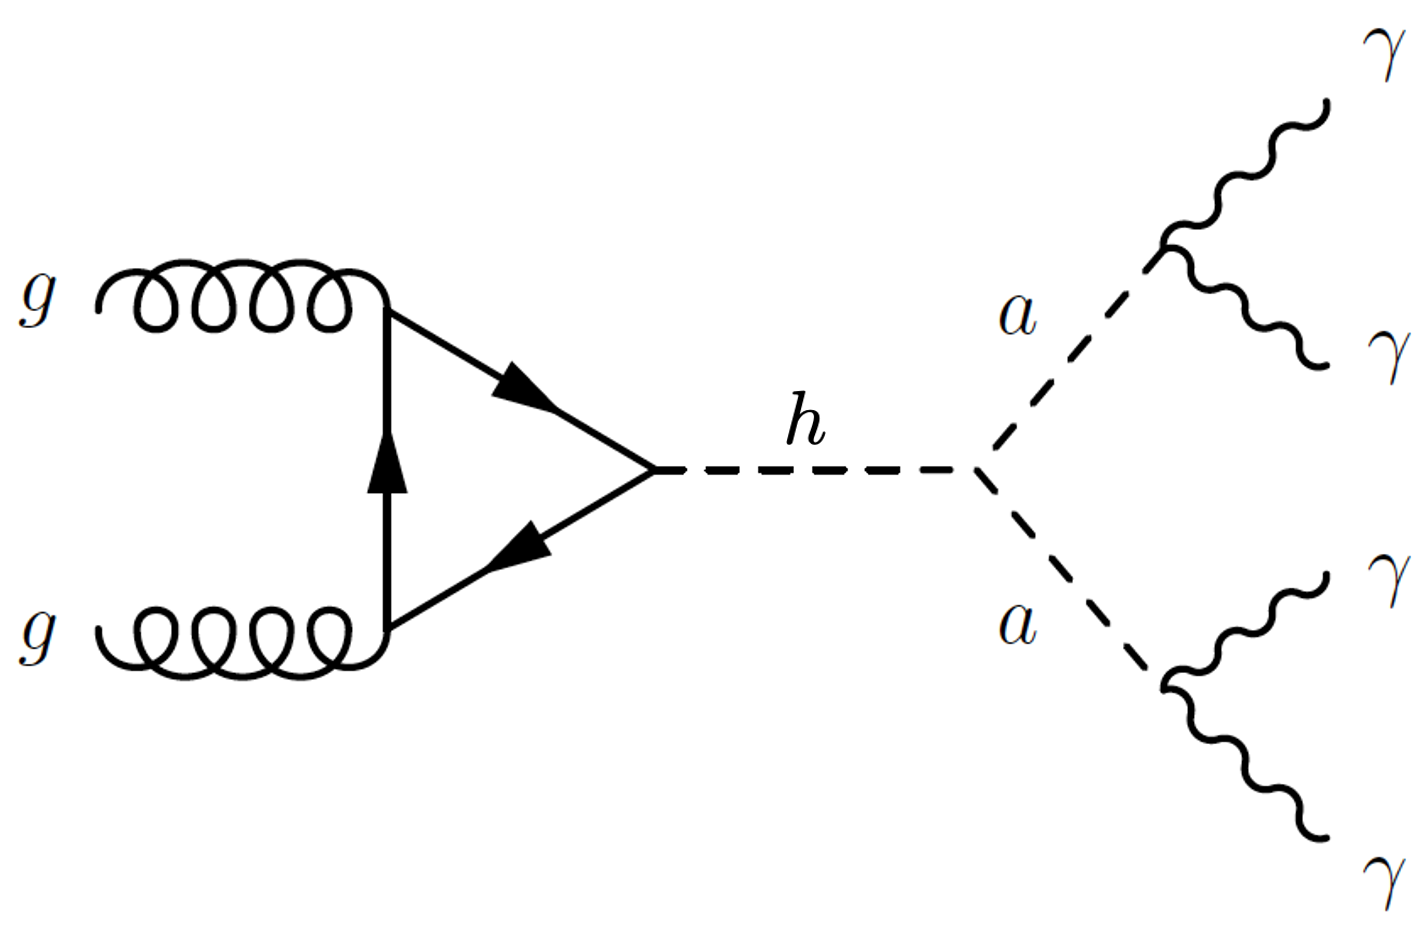
\includegraphics[width=0.45\linewidth]{figures/h4g-feynman-diagram.png}
   \caption{Tree-level Feynman diagram of $h\rightarrow aa \rightarrow \gamma\gamma\gamma\gamma$ for the gluon fusion Higgs production mode.}
   \label{fig:h4g-feynman-diag}
\end{figure}

Some models predict the existance of a light pseudoscalar boson, e.g., models with at least one extra Higgs doublet -- that is, an SU(2)\textsubscript{L} doublet \cite{Curtin_2014}. An interesting process in many of these models is the 125 GeV SM Higgs boson decay to two pseudoscalars. The tree level Feynman diagram for a Higgs boson decaying to two pseudoscalars with a four photon final state is shown in Fig \ref{fig:h4g-feynman-diag}. Given the current limits and exclusions, a large phase space remains for these decays thus a search for this BSM process can be fairly model agnostic.\par

Depending on the mass of $a$, the decay $a\rightarrow \gamma\gamma$ may have three topologies. For $m_{a} > 15$ GeV, the photons are fully resolved, i.e., angular distance, $\Delta R = \sqrt{(\Delta \eta)^2 + (\Delta \phi)^2}$, is greater than $0.2$. For $m_{a} < 15$ GeV, the opening angle of the photon pairs may be too small to resolve, yielding either a false two or three photon signal. In this analysis, we will be focusing on the fully resolved final state topology and only the gluon fusion Higgs production mode will be considered. These requirements, along with other exclusion limits to $m_{a}$, allow for a search for pseudoscalars with a mass range of $15 < m_{a} < 62$ GeV.\par


\section{LHC and CMS}
\begin{figure}
   \centering
   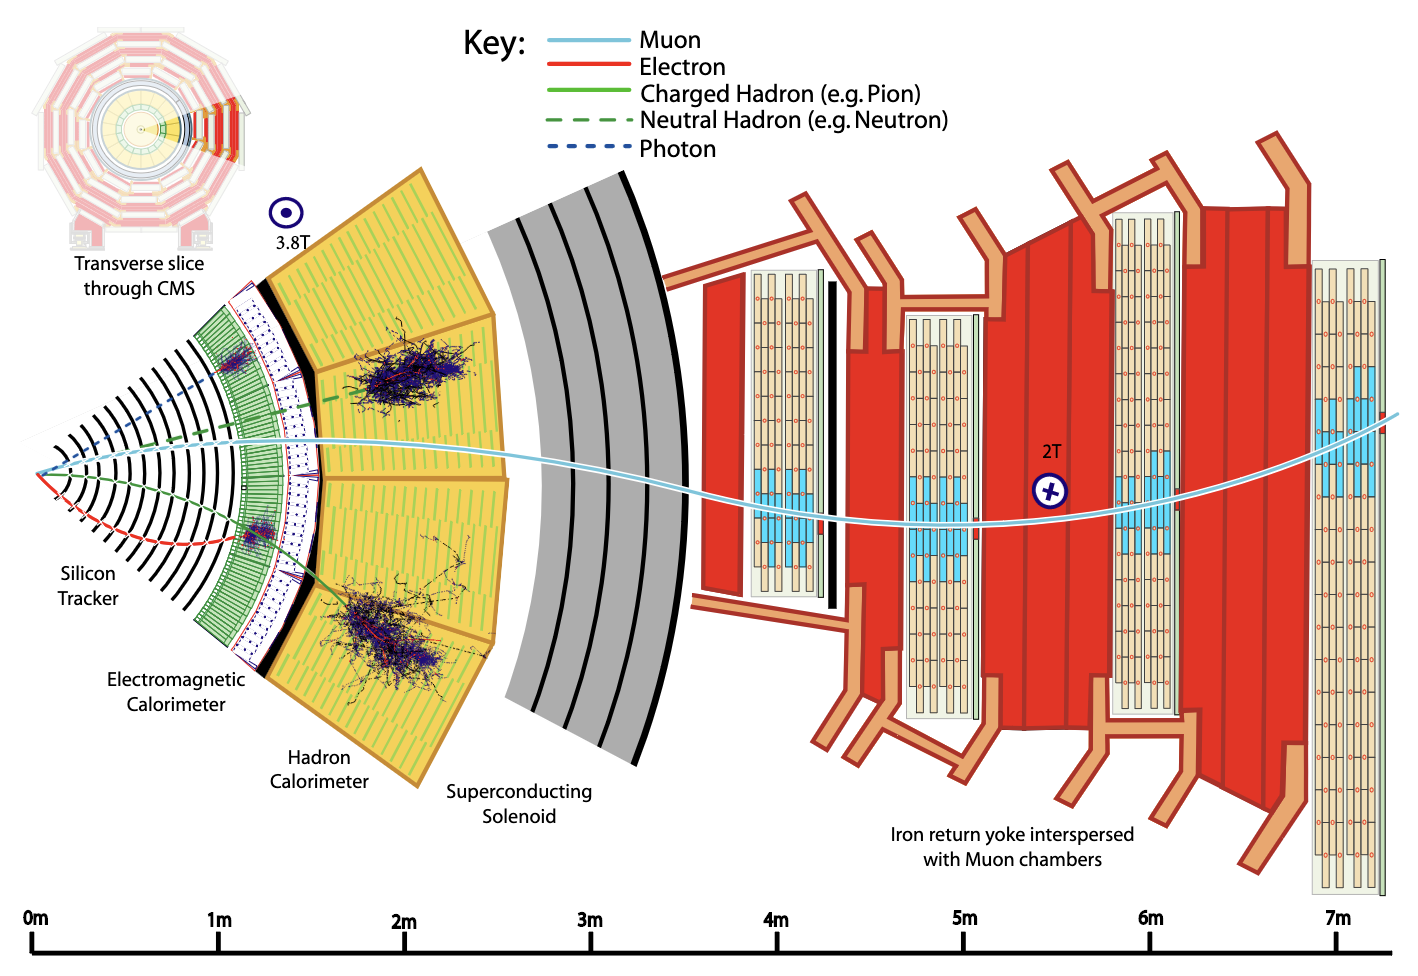
\includegraphics[width=0.8\linewidth]{figures/CMSslice_whiteBackground.png}
   \caption{Slice showing CMS sub-detectors and how particles interact in them \cite{particle_flow_2017}.}
   \label{fig:cms-subdetectors}
\end{figure}

The Large Hadron Collider (LHC) is a proton-proton collider and the world's largest particle accelerator, located on the border of France and Switzerland. It is 27 kilometers in circumference and consists of superconducting dipoles and quadrupoles, for bending and focusing the beams, respectively. The LHC currently operates at a center-of-mass energy of $13.6$ TeV with a nominal instanteous luminosity of $10^{33}\, \text{cm}^{-2}\, \text{s}^{-1}$. There are two general purpose detectors at the LHC: CMS and ATLAS.\par

The Compact Muon Solenoid (CMS) detector is a hermetic, general purpose detector along the ring of the Large Hadron Collider (LHC). CMS is composed of several sub-detectors, each designed to collect data on a specific part of a proton-proton collision event, and a superconducting solenoid at a field strength of $3.8$ T. A schematic of these sub-detectors is shown in Fig. \ref{fig:cms-subdetectors}. The main sub-detectors of CMS are, from the beam line outwards, the silicon tracker (pixel and strip), the electromagnetic calorimeter, the hadronic calorimeter, and the muon chambers \cite{CMS_Collaboration_2008}.\par

Recording a collision event requires each of these subsystems to detect different parts of the event. Many particles are created during a collision with many decaying to even more. These particles first pass through the silicon tracker, which detects charged particles as tracks, and then through the ECAL. The ECAL detects electromagnetically charged particles with lead tungstate crystals and is optimized for photons and electrons. Photon and electron energy is completely measured, but charged hadrons, while they do produce a shower, pass through. The particles enter the HCAL, a sampling calorimeter, and produce showers. Charged and neutral hadrons are contained in the HCAL, but any remaining particles, namely muons, continue through the magnet to interact with the muon chambers.\par

\subsection{ECAL}
% The silicon tracker is made of two types of solid-state devices, pixels and strips. The silicon pixels are closest to the interaction point and are used to measure the momentum of the charged particles in an event. Next are the silicon strips, larger solid-state devices that are slightly further away from the interaction point. These strips are interlaced in several layers such that they can still provide a fairly good picture of a charged particle's motion even though they are individually less precise than the pixels. Additional layers of both pixels and strips have been added since the start of the LHC.\par

The ECAL is a homogeneous calorimeter and composed of  ${\sim} 75,000$ scintillating PbWO\textsubscript{4} crystals in two parts: the barrel (EB) and the endcaps (EE), in $\eta$ ranges $|\eta| < 1.48$ and $1.48 < |\eta| < 3.00$, respectively. The PbWO\textsubscript{4} crystals measure the energy of any electromagnetically charged particle passing through them, albeit designed for optimal performance with electrons and photons. The crystals were chosen for their Moli\`ere radius and response time, i.e., a crystal contains 90\% of a shower's deposition on average and the crystal is destructive to signals at a rate consistent with collisions. Unlike the barrel section, the endcaps have an additional preshower component in two layers positioned in front of the crystals: lead and silicon, the silicon strip detectors used to detect neutral pion decays.\par

Each crystal in the ECAL has photodetectors attached it: two avalanche photodiodes for crystals in the barrel and one vacuum phototriode for crystals in the endcap. These photodetectors are connected to the on-detector electronics with each trigger tower (corresponding to $5 \times 5$ crystals) consisting of five Very Front End boards, one Front End board, several Gigabit Optical Hybrids boards, one Low Voltage Regulator board, and a motherboard. Part of my technical contribution is working on the upgrade of the on/off-detector electronics for Phase II. I am involved in writing software for hardware tests under nominal conditions and test beams. These systems are also involved in calibrating the ECAL; there is a bias voltage over the photodetectors and measurements of this bias are used in noise reduction. A laser system is also employed to monitor crystal transparency due to radiation effects and to calibrate crystal response.\par

% Continuing outwards, the next sub-detector is the hadronic calorimeter (HCAL). The HCAL is a sampling calorimeter and composed of layers of brass absorbers and plastic scintillators, which are used to identify the hadronic parts of a collision. The brass absorbers, along with steel plates, produce hadronic showers while the scintillating material measures the energy of these showers. The HCAL is also comprised of a barrel component and an endcap component in a similar manner to the ECAL. There are also several extra components to ensure that HCAL is hermetic: a forward component at high $\eta$ and an outer barrel sitting just outside of the solenoid. The radial size of these components is determined by the optimal number of radiation lengths required to minimize punch-through of hadronic showers into the muon chambers.\par

% The final and outermost component of the CMS detector is the muon chambers. Muons play an integral part in event reconstruction and their detection was a major design consideration of the CMS detector. Similarly to the other sub-detectors, the muon chambers have barrel and endcap components. In the barrel region, the magnetic field is uniform and the muon flux is low; this allows for the use of drift tubes. In the endcap regions, the magnetic field is non-uniform and the muon flux is high so a more robust system of cathode strip chambers is used. A dedicated trigger system was added to both the barrel and endcap regions in the form of resistive plate chambers, which can tag the time of an muon interaction much faster than the $25\, \mathrm{ns}$ bunch crossing rate.\par

% A full explanation of the entire CMS detector is available in an overview paper published around the start of the LHC \cite{CMS_Collaboration_2008}.\par

\subsection{Object Reconstruction}
Translating the raw hits in the detector into usable objects is a crucial step in reconstructing a collision event. CMS uses an algorithm called \textit{Particle Flow} (PF) to reconstruct objects for physics analysis \cite{particle_flow_2017}. Clustering and other reconstruction techniques create PF elements from the raw hits in the detector. These PF elements are run through a link algorithm that connects the PF elements from different sub-detectors while restricting the linking of PF elements to nearest neighbors in the $(\eta, \phi)$ plane, where $\eta$ refers to pseudo-rapidity and $\phi$ refers to azimuthal coordinate in the detector.\par

The first step is reconstructing muons by matching tracks in the muon chambers with tracks in the inner tracker while imposing restrictions on calorimeter deposits. Once muons are reconstructed, all of the muon PF elements are masked for the next set of objects; a similar masking step occurs for all PF elements after reconstruction. Electrons and isolated photons, i.e., photons without significant energy deposits in their vicinity, are then reconstructed by linking their tracks (or lack thereof), clusters in the ECAL, and lack of clusters in the HCAL; a Gaussian shower profile is used to assign the energy to clusters in the ECAL which is necessary for more complex event topologies with overlapping clusters. Proper understanding of shower shape in clusters is important for the ECAL since electrons and photons have a different shower shape than charged and neutral hadrons in the crystals \cite{egamma_reco_2021}. A multivariate analysis technique (MVA) is used to distinguish prompt photons from jets using information regarding the photon's shower shape, isolation, energy, and $\eta$.  A similar process is carried out for charged hadrons, with the addition of clusters in the HCAL and a calorimetric energy resolution cut on track $p_T$. Remaining PF elements are subject to the cross-identification of charged hadrons, neutral hadrons, and non-isolated photons/electrons, arising from parton fragmentation, hadronization, and decays in jets. These reconstructed objects are then used as inputs to jet reconstruction algorithms, e.g., anti-$k_T$.\par

\section{Previous Studies}
Previous studies have been done that include a Higgs boson decaying to two pseudoscalars, then each pseudoscalar decaying to two photons, as well as other final states. The precursor to this proposed analysis is the most recent study of the same process, i.e., the CMS Run 2 analysis of $h\rightarrow aa \rightarrow \gamma\gamma\gamma\gamma$, where the photons are fully resolved and the pseudoscalar mass range is $15 < m_a < 62$ GeV. The aforementioned Run 2 analysis utilized $132\, \mathrm{fb}^{-1}$ of data from the CMS detector and set the strictest limits on the process' production cross section to date. Run 2 lasted from late 2015 through 2018, although the nominal dataset contains data from 2016--2018.\par

\subsection{Advancements on Previous Studies}
Advancements can be made relative to the Run 2 analysis in several ways. An increase in statistics of $50-100\%$ could allow for this analysis to set even stricter limits on the cross section times branching fraction, given by $\sigma(pp \rightarrow h) \times \mathrm{Br}(h\rightarrow aa \rightarrow \gamma\gamma\gamma\gamma)$. The previous analysis reported an impact of ${\sim}1\%$ from systematic uncertainties, meaning that an increase in statistics would be an almost direct improvement to analysis sensitivity \cite{Run2_analysis}. The true increase in statistics is heavily dependent on both CMS and LHC schedules, but the  availability of 2022 and 2023 data by early-2024 suggest an increase in statistics of about $50\%$ \cite{PC_CMS_Week}. It may also be possible to reduce the ${\sim}1\%$ impact from statistical uncertainties since Run 3 data is expecting a gain of $\sqrt{2}$ times precision on Run 2.\par

A new methodology may also be employed to increase sensitivity with respect to the previous analysis. It may be possible to utilize a different type of machine learning (ML) technique, previously a boosted decision tree (BDT), to train an event selection model; the new technique would likely use deep learning to construct the model. Deep learning models may require more events than are available to be viable as these models only surpass BDTs when trained with at least ${\sim} 100\mathrm{k}$ events \cite{DNN_May}. While the expected yield post all selections from $132\, \mathrm{fb}^{-1}$ of data is nowhere near the ideal $100\mathrm{k}$ events, the number of events used to train a ML model is significantly higher since training happens before the categorization step that involve a cut on events. Any lack of statistics required for a deep learning model can be alleviated by two things: artifically increasing signal statistics by generating additional signal samples, which is more computationally expensive, and including Run 3 data in the proposed analysis since the background for this analysis is data driven. It is yet unclear whether this analysis will be a partial Run 3 or a combination of the full Run 2 and partial Run 3 data; regardless, the increase in statistics will improve the viability of utilizing a deep learning model instead of a BDT.\par

A major difference between this proposed analysis and its inspiration, the Run 2 analysis, changes the tools necessary to search for this process. Arguably, the most significant change is the use of the newer nanoAOD data format as opposed to the use of the miniAOD data format. On one hand, it limits the use of certain event selection techniques and, on the other, requires an entirely new analysis framework. An analysis framework handles everything from loading samples to processing cuts and selections to applying systematic uncertainties to samples. The frameworks used in analyses with miniAOD and nanoAOD are common to the $h\rightarrow\gamma\gamma$ group: Flashgg for miniAOD, like the Run 2 analysis, and HiggsDNA for nanoAOD, like this proposed analysis \cite{Flashgg, HiggsDNA}.\par

\subsection{New Framework: HiggsDNA}
The new analysis framework HiggsDNA (Higgs to Diphoton NanoAOD Framework), produced by the $H \rightarrow \gamma\gamma$ group, is built on Coffea, a tool for processing nanoAOD samples \cite{lindsey_gray_2023_8408347}. HiggsDNA utilizes Coffea processors and uses a columnar-based approach rather than an event-based approach to accessing data; current columnar-based analysis is significantly faster than its event-based counterpart. Coffea processors enable the efficient use of cuts across an entire column (in the context of a flat tree), e.g., a simple $p_T$ cut is now applied simultaneously to the entire column instead of looping through each event and applying the cut per event.\par

A proof of concept is needed before applying HiggsDNA to a Run 3 analysis so a partial recreation of the Run 2 analysis is underway. The recreation is for 2018 only and there is an attempt to keep any necessary modifications to a minimum; all cuts, BDT input variables, and other Run 2 specific parameters are unchanged. It should be noted that all samples for the year 2018 from the Run 2 analysis have been converted from miniAOD to nanoAOD with some additional, non-standard branches that are used by the $H \rightarrow \gamma\gamma$ group; the subset of these branches that are required for HLT mimicking cuts are \textit{chargedHadronIso}, \textit{trkSumPtHollowConeDR03}, and \textit{pfPhoIso03}, and \textit{fixedGridRhoAll} for pileup corrections. These branches are included in newer versions of nanoAOD, but are not included in the 2018 Ultra Legacy (UL) samples since UL are currently stored as nanoAODv9. In the case of 2022-onwards data, the centrally produced nanoAOD samples should be nanoAODv12, which has all but \textit{chargedHadronIso}. Unfortunately, the use of even this modified nanoAOD makes it impossible to utilize a BDT to determine the correct primary vertex, as was standard in the Run 2 analysis. The $h\rightarrow \gamma\gamma$ primary vertex can occasionally differ from the standard CMS primary vertex ($\mathrm{max}\,\Sigma p_T$). The lack of a vertex BDT additional step in the event selection process reduces the Higgs mass resolution by about $3\%$, although this may be alleviated by the increase in precision in Run 3. Lastly, scaling and smearing corrections for photons have not yet been applied in this analysis as there is a prerequisite configuration file that has yet to be produced.\par

\section{Signal and Background}
The signal samples are simulated $H \rightarrow aa \rightarrow \gamma\gamma\gamma\gamma$ Monte Carlo (MC) with a pseudoscalar mass range of $15 < m_a < 60$ GeV in steps of $5$ GeV and a Higgs boson mass of 125 GeV. These samples only consider the gluon fusion production mechanism of the Higgs boson and were generated using MADGRAPH5\_aMC@NLO for the previous analysis. The 2018 signal samples were converted to nanoAOD in the manner prescribed above for the proposed analysis. New signal MC will be needed for the Run 3 analysis and are expected to be generated in a substantially similar manner. Corrections to the signal MC to achieve a better agreement between data and simulation will be applied and are dependent on detector performance in a given data-taking year. Corrections come in the form of photon smearing and scaling, among others, however, they have yet to be applied to the signal MC used in the proof-of-concept study.\par

The Run 2 analysis has shown that a MC-based background was not viable since the MC available from the standard $H \rightarrow \gamma\gamma$ analysis (QCD, $\gamma + \mathrm{jets}$, and $\gamma\gamma + \mathrm{jets}$) suffered from low statistics, and thus very large event weights, after requiring the presence of four photons in an event. The same technique will be used in this analysis to avoid the same problems. The data driven background utilizes a technique similar to hemisphere mixing to remove the presence of any signal and artificially create the background shape \cite{hemisphere_mixing}. This technique is called \textit{event mixing} and is a simplification of the hemisphere mixing procedure. The methodology of event mixing varies between columnar-based analysis and event-based analysis; columnar-based event mixing is significantly less computationally expensive. Event mixing shuffles the photons in an event with the photons from consecutive events, modulo the number of events. Considering photons in descending order by $p_T$ for an event $N$, the first photon is unchanged in event $N$, the second photon is replaced with the photon from event $N+1$, the third is replaced with the photon from event $N+2$, and the forth is replaced by the photon from event $N+3$.\par

The event mixed background samples were generated in several steps. 2018UL data samples were converted from miniAOD to nanoAOD with the necessary extra branches, thus diverging slightly from the central 2018UL data samples and the 2018 non-UL samples used in the full Run 2 analysis. The resulting UL samples then underwent the event mixing procedure before being processed in the event selection step. Event mixed background samples, in nanoAOD format, were not stored as a space saving measure. Instead, event mixing is calculated for on the fly before applying selections.\par
% Bias studies will be performed on the newly generated background samples as was done in the Run 2 analysis.


\section{Event Selection}
% general overview of what is needed to select signal/background events
% Delta-M procedure for pseudoscalar->gamma+gamma (related to hemisphere mixing)
% mention cuts and selections (HLT mimicking, additional cuts on pseudoscalars and Higgs mass), the BDT model, and BDT categorization.
% even/odd (testing/training, respectively) events into BDT and signal modelling
Signal events are extracted from data via high level trigger (HLT) mimicking cuts, additional cuts and selections on the pseudoscalars and the four photon object, a BDT model to discriminate signal/background, and a categorization procedure based on BDT score. Events are selected using an HLT path optimized for the low mass diphoton Higgs boson search. The HLT path and associated mimicking cuts for 2018 are shown in Table \ref{tab:hlt_cuts_2018}. It is important to note that these trigger paths, cuts, and selections will all be evaluated, and potentially changed, for the Run 3 analysis. All of the listed criteria for the 2018 proof-of-concept study is taken from the Run 2 analysis, where optimization of cuts has already been performed.\par

% mention that I will do tag and probe with Z->ee events eventually
The HLT is applied to both simulated and data samples. Events are also required to contain at least one diphoton candidate. Additional, more strict cuts are then applied to the photons from the diphoton candidate. Both photons must pass either $R_9 > 0.8$, Charged Hadron Isolation $<20$ GeV, or (Charged Hadron Isolation)/$p_T < 0.3$ if $p_T > 14$ GeV and $H/E < 0.15$. Photons must also pass an electron veto; a photon candidate is rejected if its supercluster has a matching electron track with at least one hit in the pixel tracker. The cuts on diphoton candidates will be referred to as pre-selections in this analysis.\par

Events that consist of at least one diphoton which pass the pre-selection requirements are subject to additional selections relating to the pseudoscalars and their daughter photons. The events must contain at least four photons where, in descending order of $p_T$, the leading two photons must pass $\gamma_1$ $p_T > 30$ GeV and $\gamma_2$ $p_T > 18$ GeV while the remaing two photons must pass a minimum $p_T$ threshold of $p_{T} > 15$ GeV. There is some overlap with the pre-selections, however the additional cut of 15 GeV on $\gamma_{3/4}$ is necessary to achieve maximal performance from the event selection BDT. All photons must also fall within the tracker fiducial region, i.e., $|\eta| < 2.5$, and not within the EB-EE gap, $1.442 < |\eta| < 1.552$, where photon reconstruction is suboptimal. Finally, there is a restriction on the mass of the four photon object of $110 < m_{\gamma \gamma \gamma \gamma} < 180$ GeV. The signal region in this analysis is defined as $115 < m_{\gamma \gamma \gamma \gamma} < 135$ GeV while the sideband region is defined as the union of $110 < m_{\gamma \gamma \gamma \gamma} < 115$ GeV and $135 < m_{\gamma \gamma \gamma \gamma} < 180$ GeV.

After applying cuts, the pseudoscalars need to be reconstructed from the four photons in an event. In the case of an event with more than four photons, the four with the highest $p_T$ are chosen. To reconstruct the pseudoscalar candidate, a technique called mass mixing is used. All combinations of the pseudoscalar candidate pairs, which each consist of two photons, are computed. To determine which set of pseudoscalar candidates is the best match, the quantity $\Delta M = |m_{a_{\gamma_{a}, \gamma_{b}}} - m_{a_{\gamma_{c}, \gamma_{d}}}|$, where $a,b,c,d \in \{1,2,3,4\}$, is calculated. This $\Delta M$ tells us which two sets of photons have the lowest absolute difference in invariant mass, i.e., the two sets with the most optimal photon pairing. The pair of pseudoscalar candidates with the lowest $\Delta M$ are chosen for each event. No cuts are applied directly to the pseudoscalar candidates.\par

\begin{table}
   \centering
   \begin{tabular}{l|c|c|c|c|c|c}
        & $E_T$ & $R_9$ & $H/E$ & $\sigma_{i\eta i\eta}$ & PF Pho Iso & Tracker Iso\\ \hline
       EB; $R_9>0.85$ & $15.0$ & $> 0.5$ & $<0.08$ & $<0.015$ & $<4.0$ & $<6.0$\\
       EB; $R_9\leq0.85$ & $15.0$ & $> 0.5$ & $<0.08$ & $<0.015$ & $<4.0$ & $<6.0$\\
       EE; $R_9>0.9$ & $15.0$ & $> 0.8$ & $<0.08$ & $<0.035$ & $<4.0$ & $<6.0$
   \end{tabular}
   \caption{Cuts mimicking the low mass diphoton Higgs boson HLT path:\\ \textit{HLT\_Diphoton30\_18R9IdL\_AND\_HE\_AN\_IsoCaloId\_NoPixelVeto}.}
   \label{tab:hlt_cuts_2018}
\end{table}
% Note: H/E is energy in HCAL over energy in ECAL

\subsection{Event Selection BDT}
The event selection BDT is a 4-photon event classifier used to distinguish between signal-like and background-like events. Training samples are produced using signal MC and data. Data samples are processed to produce event mixed background samples. Then signal MC and event mixed background samples have all analysis selections applied. An additional step of adding a variable, $m_{Hyp}$, corresponding to the hypothesis mass point is done for both samples. For the event mixed background sample, $m_{Hyp}$ is a flat distribution with discrete peaks at each pseudoscalar mass point, by construction. When using the trained model to make predictions, $m_{Hyp}$ and any variables that depend on it are recalculated as a discrete peak at the hypothesis mass point.\par

The result is samples of pure signal events and pure background events. These signal and background samples are used as inputs to the 4-photon BDT, where a subset of relevant variables are used to train the model. Only one model is trained for all mass points; the $m_{Hyp}$ variable, and other variables dependant on it, allow the model to distinguish the hypothesis mass point when computing predictions. The training variables are listed below:\par

\begin{itemize}
   \item $\gamma_{1-4}$ MVA ID
   \item $a_{1,2}\; p_T$
   \item $\frac{\Delta R(a_{1}, a_{2})}{m_{\gamma\gamma\gamma\gamma}}$
   \item $m_{a1} - m_{a2}$
   \item $\cos\theta_{a\gamma}$ where $\theta_{a\gamma}$ is defined as the angle between the leading photon coming from the leading pseudoscalar and the direction of $a\rightarrow\gamma\gamma$
   \item $\frac{m_{a1\,RECO} - m_{a\, Hyp}}{m_{\gamma\gamma\gamma\gamma}}$
   \item $\frac{m_{a2\,RECO} - m_{a\, Hyp}}{m_{\gamma\gamma\gamma\gamma}}$
\end{itemize}


There is some disagreement between data and background distributions of the training variables, thus a multi-dimensional, per-event reweighting is performed on the entire $m_{\gamma\gamma\gamma\gamma}$ range. The reweighting is calculated using the ratio of event mixed background and data in the $m_{\gamma\gamma\gamma\gamma}$ sideband region. The variables $\Delta$R($a_1,a_2$), $a_{1,2}\; p_T$, and $m_{a1} - m_{a2}$ are used to calculate the per-event weights. The reweighted samples are used as input to train and test the BDT. A split on even/odd events is performed such that the training set consists of odd events and testing events consists of even events.\par


\subsection{Categorization}
Once the model is trained, it is applied to signal MC and event mixed background. All events are considered, both training and testing sets used in the previous step. A categorization optimization procedure is applied on the prediction distributions to maximize the significance for each category for a minimal number of categories. The Approximate Mean Signficance is defined in Eq \ref{eqn:ams}. It is know that the total significance increases with the number of categories, thus the number of categories is optimized such that a minimal number are created, which increases the number of signal events per category.\par

\begin{equation} \label{eqn:ams}
\text{AMS} = \sqrt{2 \left[ (S + B) \ln \left(1 + \frac{S}{B}\right) - S \right]}
\end{equation}

To better emulate the prediction distribution of real data, a 1-dimensional reweighting is performed. The new event weights are generated from the ratio of background and data in the sideband region. In order to minimize large statistical fluctuations with very fine binning but retain the high granularity, the event mixed background prediction distribution is smoothed using the \textit{SmoothSuper} function in the \textit{TGraphSmooth} class from ROOT. Before the smoothing, a cut on the BDT score is applied at $\sim 0.1$, which removes the background-like peak from the distribution, in order to improve the smoothing procedure.\par

The optimization procedure is applied and the category boundaries are generated. A requirement of at least 8 events in the data samples for the same bin is required when calculating category boundaries. Only one category was necessary in the Run 2 analysis, but that is not the case currently with this analysis. The current idea is that this is due to a combination of factors, namely a difference in the quality of the event selection BDT, the lack of scaling and smearing corrections, and the lack of a vertex BDT.\par

Finally, these category cuts are applied to the signal and event mixed background such that there is a set of samples for each category. Note that both the N-dimensional and 1-dimensional reweighting procedures do not affect real data in any way. The reweighting is used only as a tool to improve the effectiveness of the event selection BDT and the categorization optimization.\par


\section{Statistical Analysis}
\subsection{Signal Modelling} \label{sec:sig-mod}
A model of the signal shape for each nominal pseudoscalar mass point is needed. After all selections and categorization cuts are applied, only training (even) signal events are kept for the signal modelling step. A signal model is computed for the $m_{\gamma \gamma \gamma \gamma}$ distribution from each signal sample. A separate signal model is generated for each category. Note that due to current issues with the BDT, the categorization step is imperfect and thus, the signal modelling step suffers as well. It was decided to fit models with a double-sided Crystal Ball function or the sum of Gaussians however, the Gaussian is shown to fit the best. In the Run 2 analysis, a double-sided Crystal Ball function was used.\par

The order of Gaussians used to fit the $m_{\gamma \gamma \gamma \gamma}$ distribution is determined by the likelihood ratio test. The optimal order is reached when $2\Delta NLL = 2[\text{NLL}_{N} - \text{NLL}_{N+1}] \leq 0.05$, where $\text{NLL}_{N}$ is the negative log likelihood for $N$ Gaussians. NLL is computed by \textit{RooFit::minNll}. The quantity $2\Delta NLL$ follows a $\chi^2$ distribution with M degrees of freedom, where M is the difference in degrees of freedom between N+1 and N Gaussians. The ideal number of Gaussians for all pseudoscalar mass points is found to be two.\par

After signal models for nominal mass points are generated, models for intermediate mass points, e.g., $47$ GeV, are required. It is known that the $m_{\gamma\gamma\gamma\gamma}$ resolution varies smoothly as a function of $m_{a}$ \cite{Run2_analysis}. Should the variation of mass resolution between each nominal mass point be fairly small, the parameters of the nominal mass points may be used. Normalization may also be interpolated from the smooth distribution of (detector efficiency $\times$ analysis acceptance). This process for generating these intermediate mass point models is currently incomplete.\par

\subsection{Background Modelling}
A background model is used to quantify the shape of $m_{\gamma\gamma\gamma\gamma}$ resulting from non-signal events. The background shape is modelled as one of the following functions: exponentials, Bernstein polynomials, Laurent series, and power law functions. The choice of function is treated as a nuisance parameter in the likelihood fit to data. Uncertainties are accounted for with the discrete profiling method, performed by the Higgs Combine statistical analysis software \cite{discrete-profiling, higgs-combine}. The fits will be computed over the entire $110 < m_{\gamma\gamma\gamma\gamma} < 180$ GeV range. A background model will be generated for each pseudoscalar mass point. It is also worth noting that turn-on checks have not yet been performed for effects of cut(s) on BDT score on background shape.\par

\subsection{Systematic Uncertainties}
Systematic uncertainties for the Run 3 analysis are expected to be largerly similar to those of the Run 2 analysis and the low mass $h\rightarrow \gamma\gamma$ analysis. They can be split into several groups: those that affect the background estimation, those that affect the signal shape, and those that affect only the signal normalization. The tag-and-probe technique will be used to calculated efficiencies and propagate uncertaines for selections \cite{Chatrchyan2011}. As the propagation of systematic uncertainties within this analysis is largerly unexplored as of yet, further discussion will be omitted.\par

\subsection{Limits}
A signal plus background model of the $m_{\gamma\gamma\gamma\gamma}$ distribution will be produced and fit to the data using a likelihood ratio as the test statistic, entirely by the Higgs Combine software, in a similar manner to that described in Ref. \cite{higgs-search-2012}. This procedure is performed for all mass points, i.e., $15 < m_{a} < 62$ in steps of 1 GeV, where the signal model for intermediate mass points is generated following the procedure outlined in Sec. \ref{sec:sig-mod}. Upper limits on $\sigma(pp \rightarrow h) \times \mathrm{Br}(h\rightarrow aa \rightarrow \gamma\gamma\gamma\gamma)$ will be set at the 95\% confidence level, as is standard in many CMS analyses, for the entire $110 < m_{\gamma\gamma\gamma\gamma} < 180$ GeV range. Further discussion is omitted since this step has yet to be completed. The procedure for the Run 3 analysis would be substantially similar.\par
% Need to re-read about confidence intervals for the presentation!!!!!


\section{Summary}
% Overview of current analysis work
% Future plans to use Run 3 data and maybe merge with Run 2
A search for the SM Higgs boson decaying to pseudoscalars with a fully resolved, four photon final state is proposed. Many of the tools needed to perform the full analysis have been created -- adjustments for new data notwithstanding -- including a full event selection with an associated BDT, category optimization tools, and signal modelling tools for nominal mass points. The aim of a Run 3 study is to improve upon the existing Run 2 analysis limits, regardless of whether this analysis utilizes purely Run 3 data or combines Run 2 and 3. The plans for this analysis are to reach a level of acceptance of the recreation of the 2018 subset of the Run 2 analysis, achieving the previously set limits at a minimum, with the HiggsDNA framework such that we can begin working with Run 3 data. Some work is still required to complete the 2018 proof-of-concept study, but should enable a fast and smooth transistion to working with Run 3 data.\par

\newpage
\printbibliography

\end{document}